\begin{figure} [b]% "[t!]" placement specifier just for this example
	\centering
\begin{subfigure}{0.25\textwidth}
	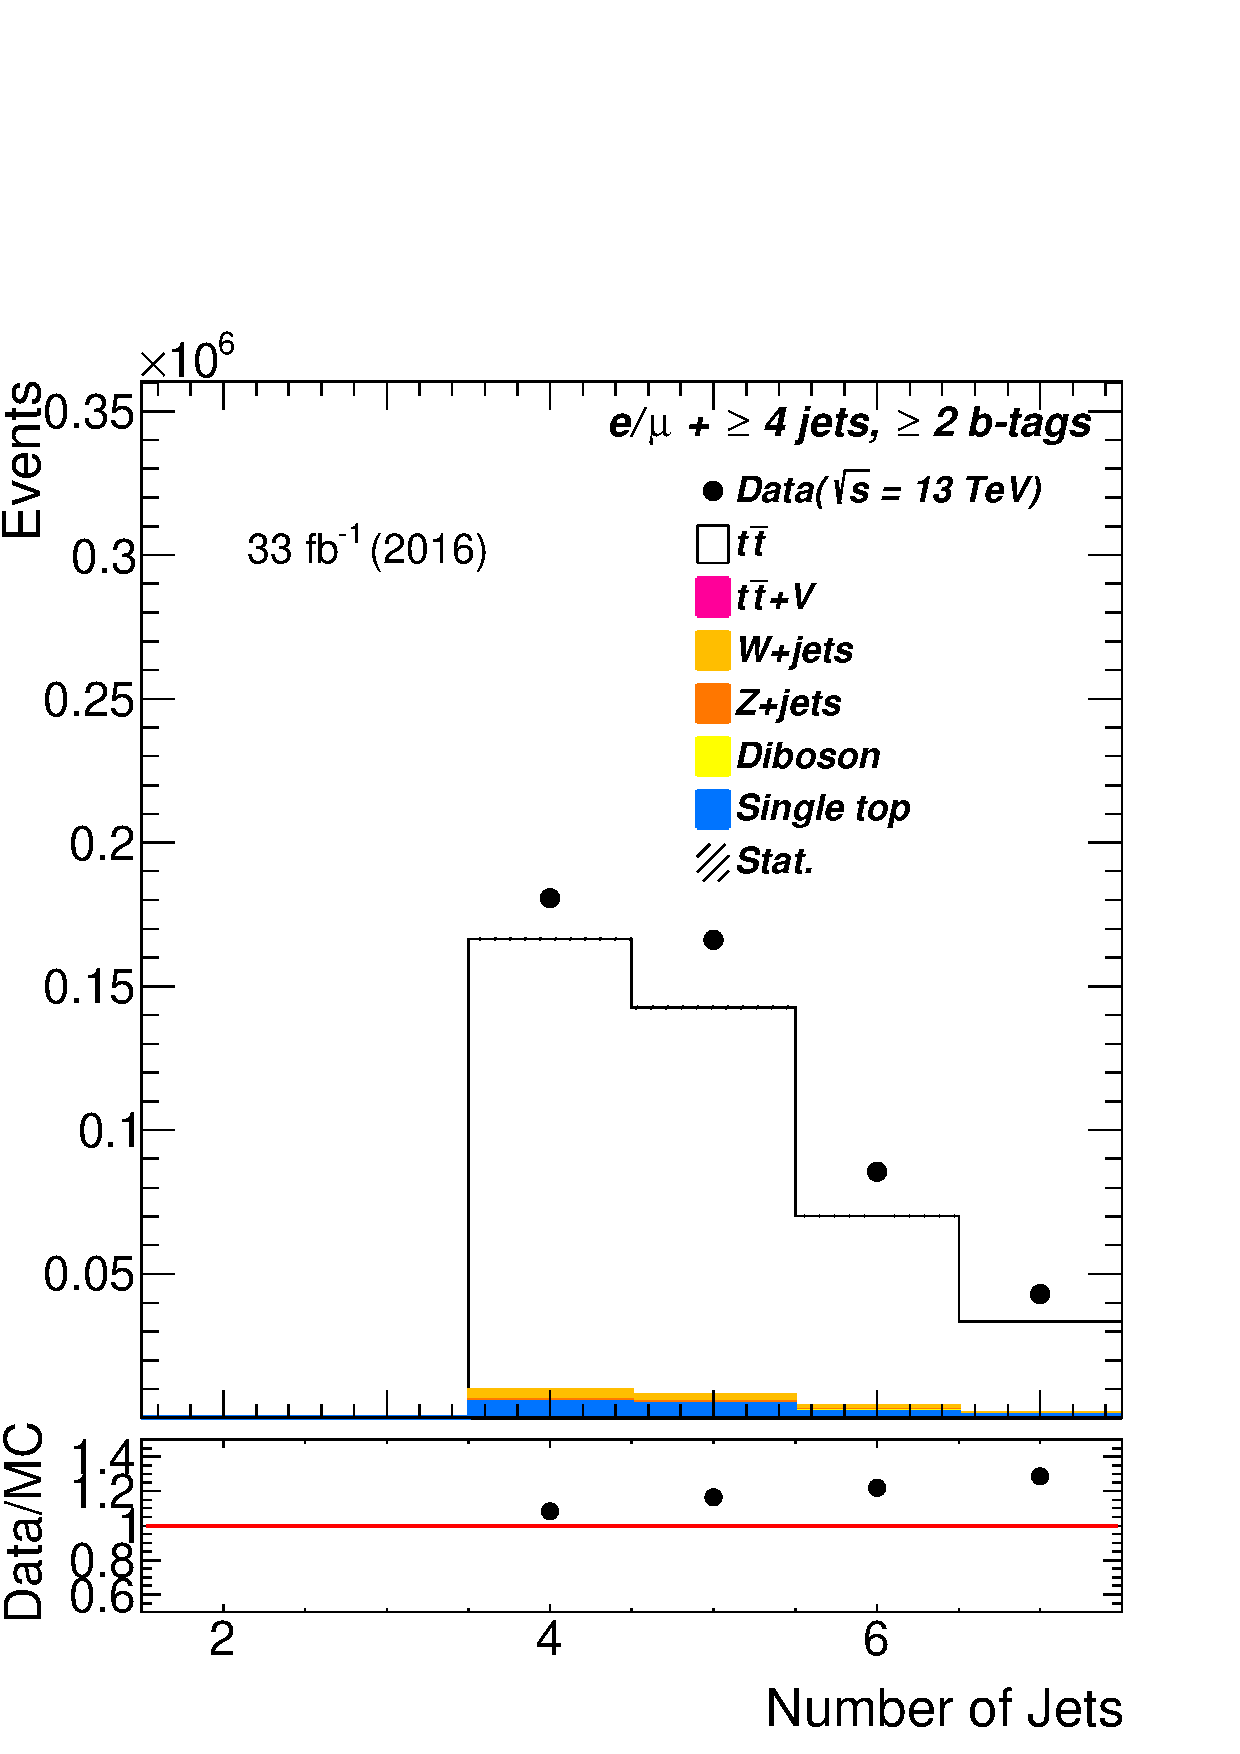
\includegraphics[width=\linewidth]{ControlPlots_emujets_2016_4incl_2incl/jet_n_emujets_2016.png}
	\caption{Number of jets.} \label{fig:Sec1}
\end{subfigure}
\hspace*{0.5cm}
\begin{subfigure}{0.25\textwidth}
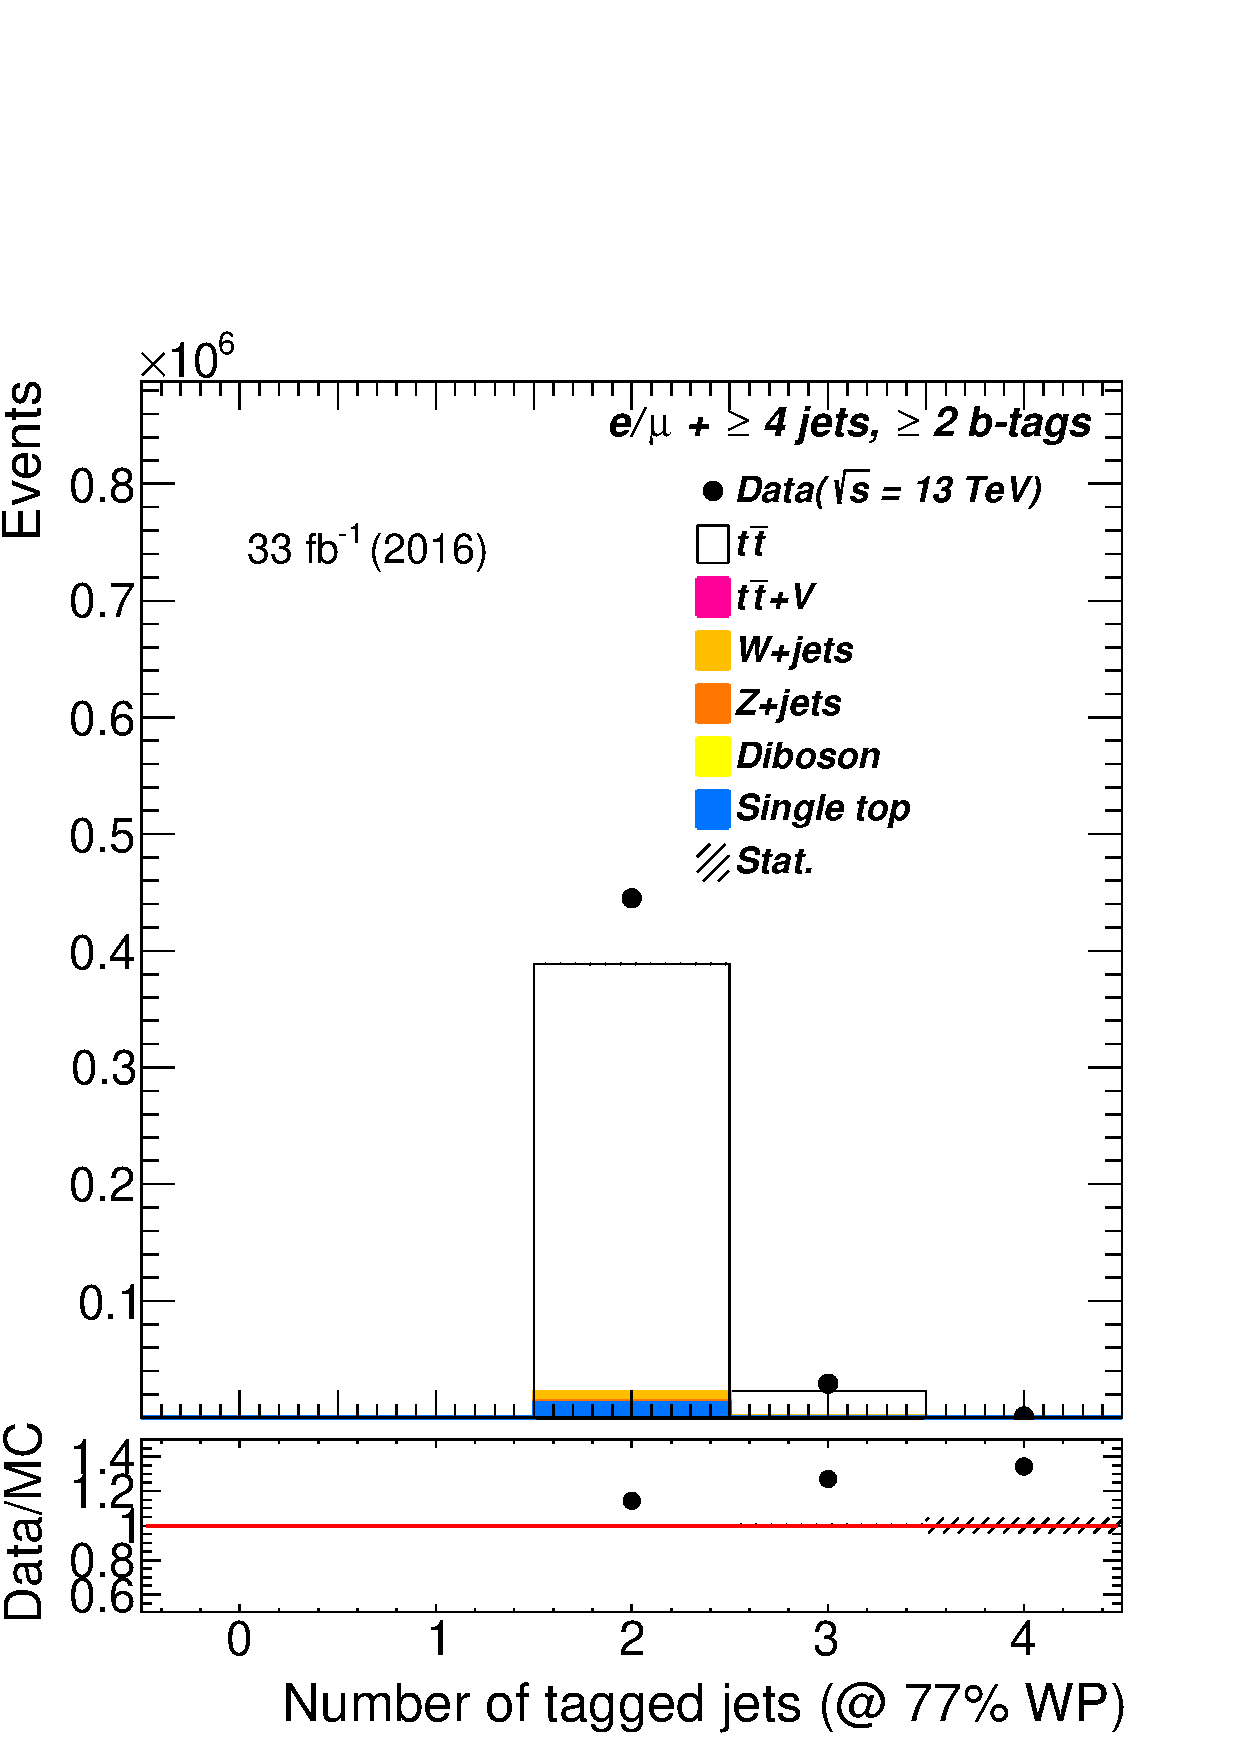
\includegraphics[width=\linewidth]{ControlPlots_emujets_2016_4incl_2incl/nBTags_emujets_2016.png}
\caption{Number of $b$-tagged jets.} \label{fig:Sec2}
\end{subfigure}
\hspace*{0.5cm}
\begin{subfigure}{0.25\textwidth}
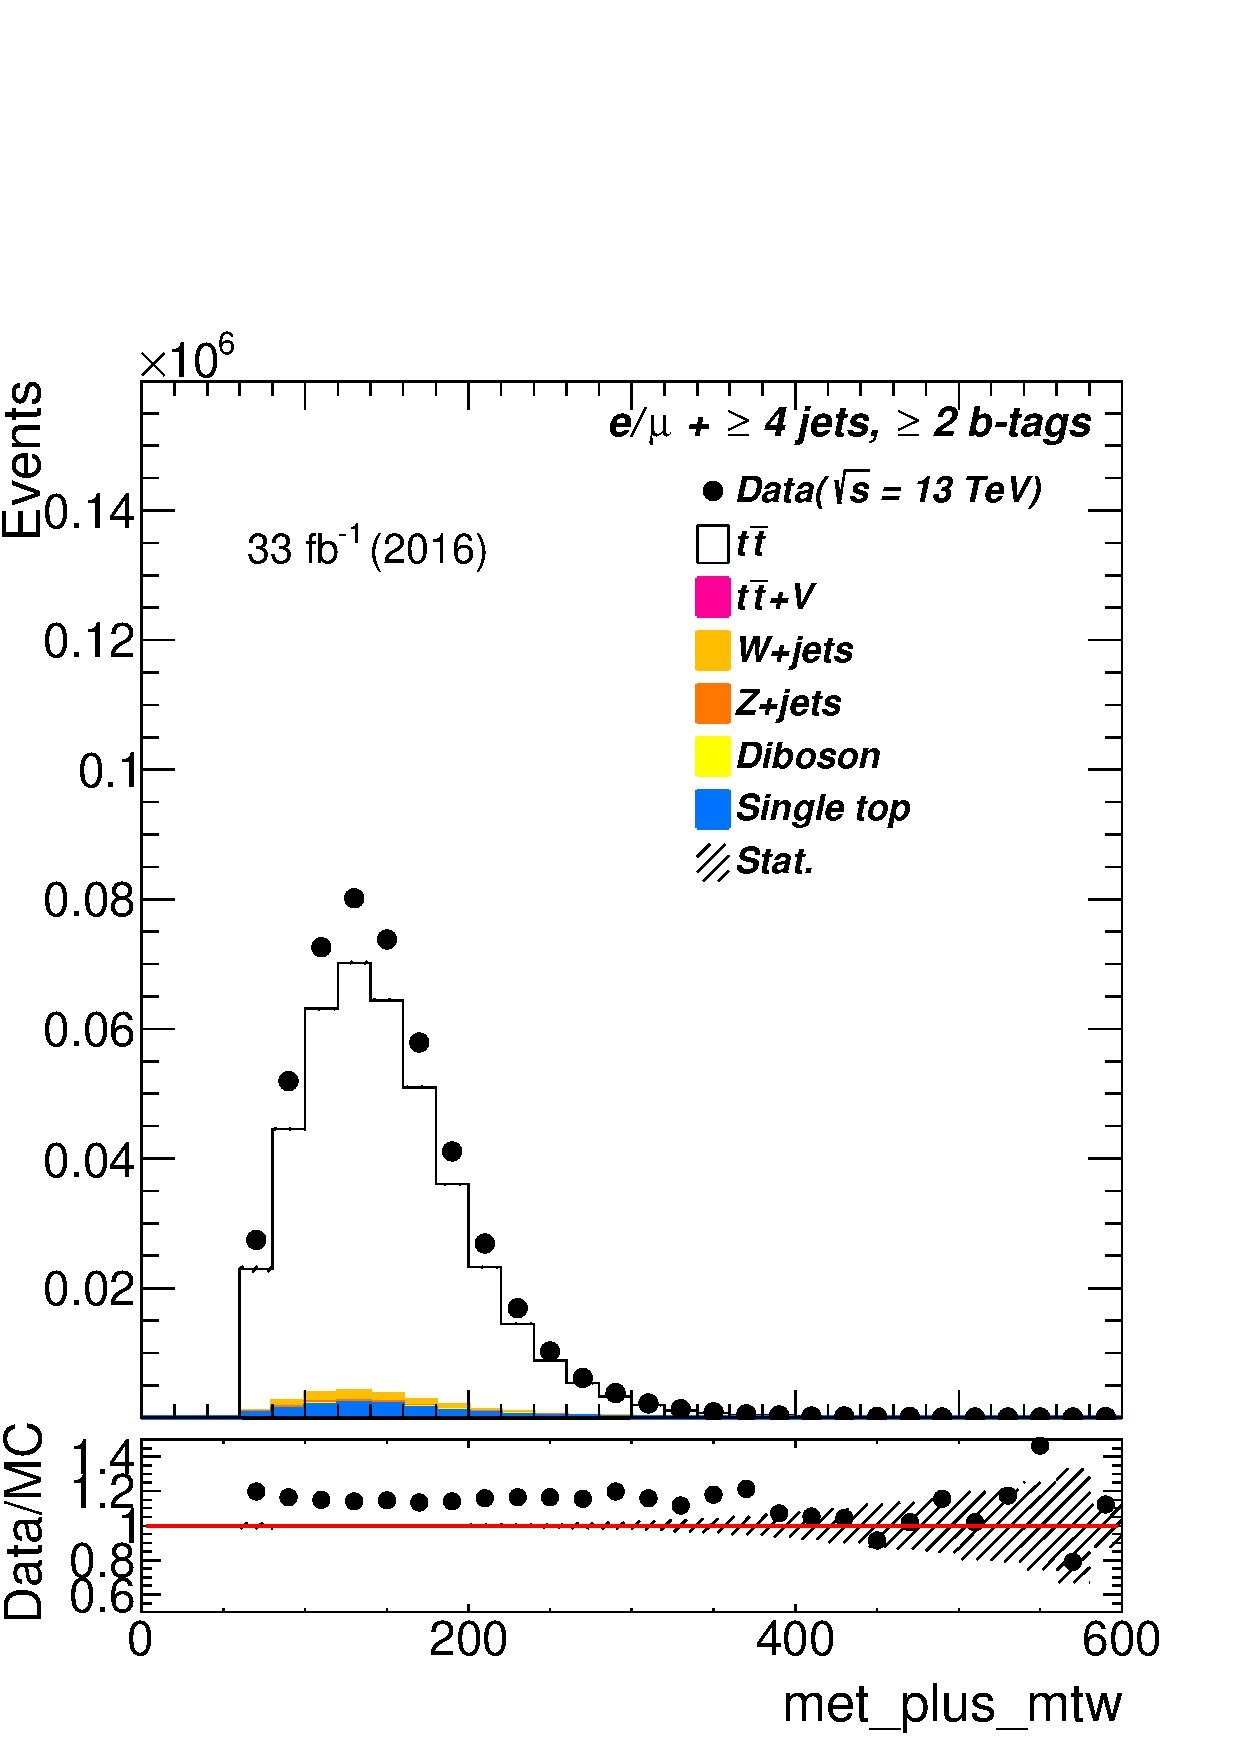
\includegraphics[width=\linewidth]{ControlPlots_emujets_2016_4incl_2incl/met_plus_mtw_emujets_2016.pdf}
\caption{$E_T^{\rm miss}$ + $W_T$-mass.} \label{fig:Sec3}
\end{subfigure}
	
	
\begin{subfigure}{0.25\textwidth}
	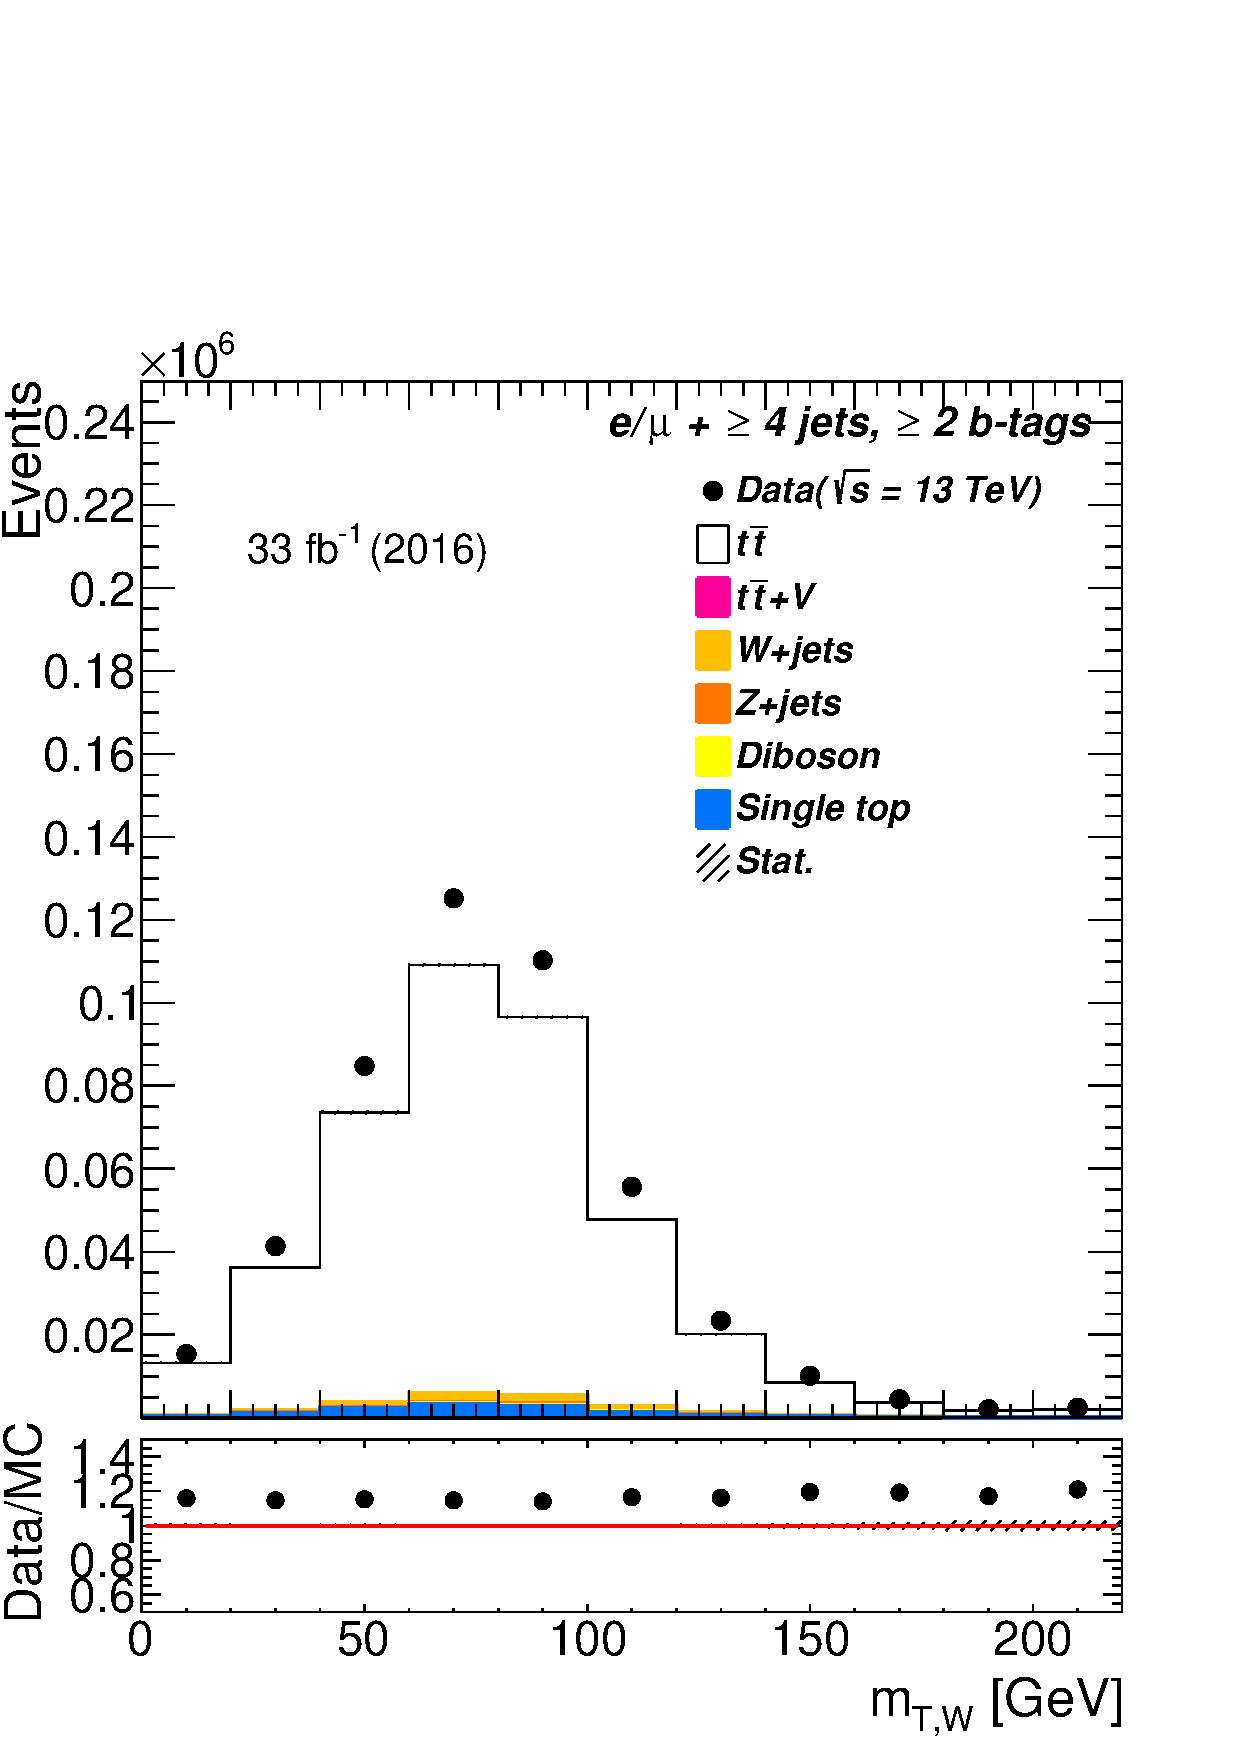
\includegraphics[width=\linewidth]{ControlPlots_emujets_2016_4incl_2incl/mtw_emujets_2016.png}
	\caption{Leptonic  $W_T$-mass.} \label{fig:Sec4}
\end{subfigure}
\hspace*{0.5cm}
\begin{subfigure}{0.25\textwidth}		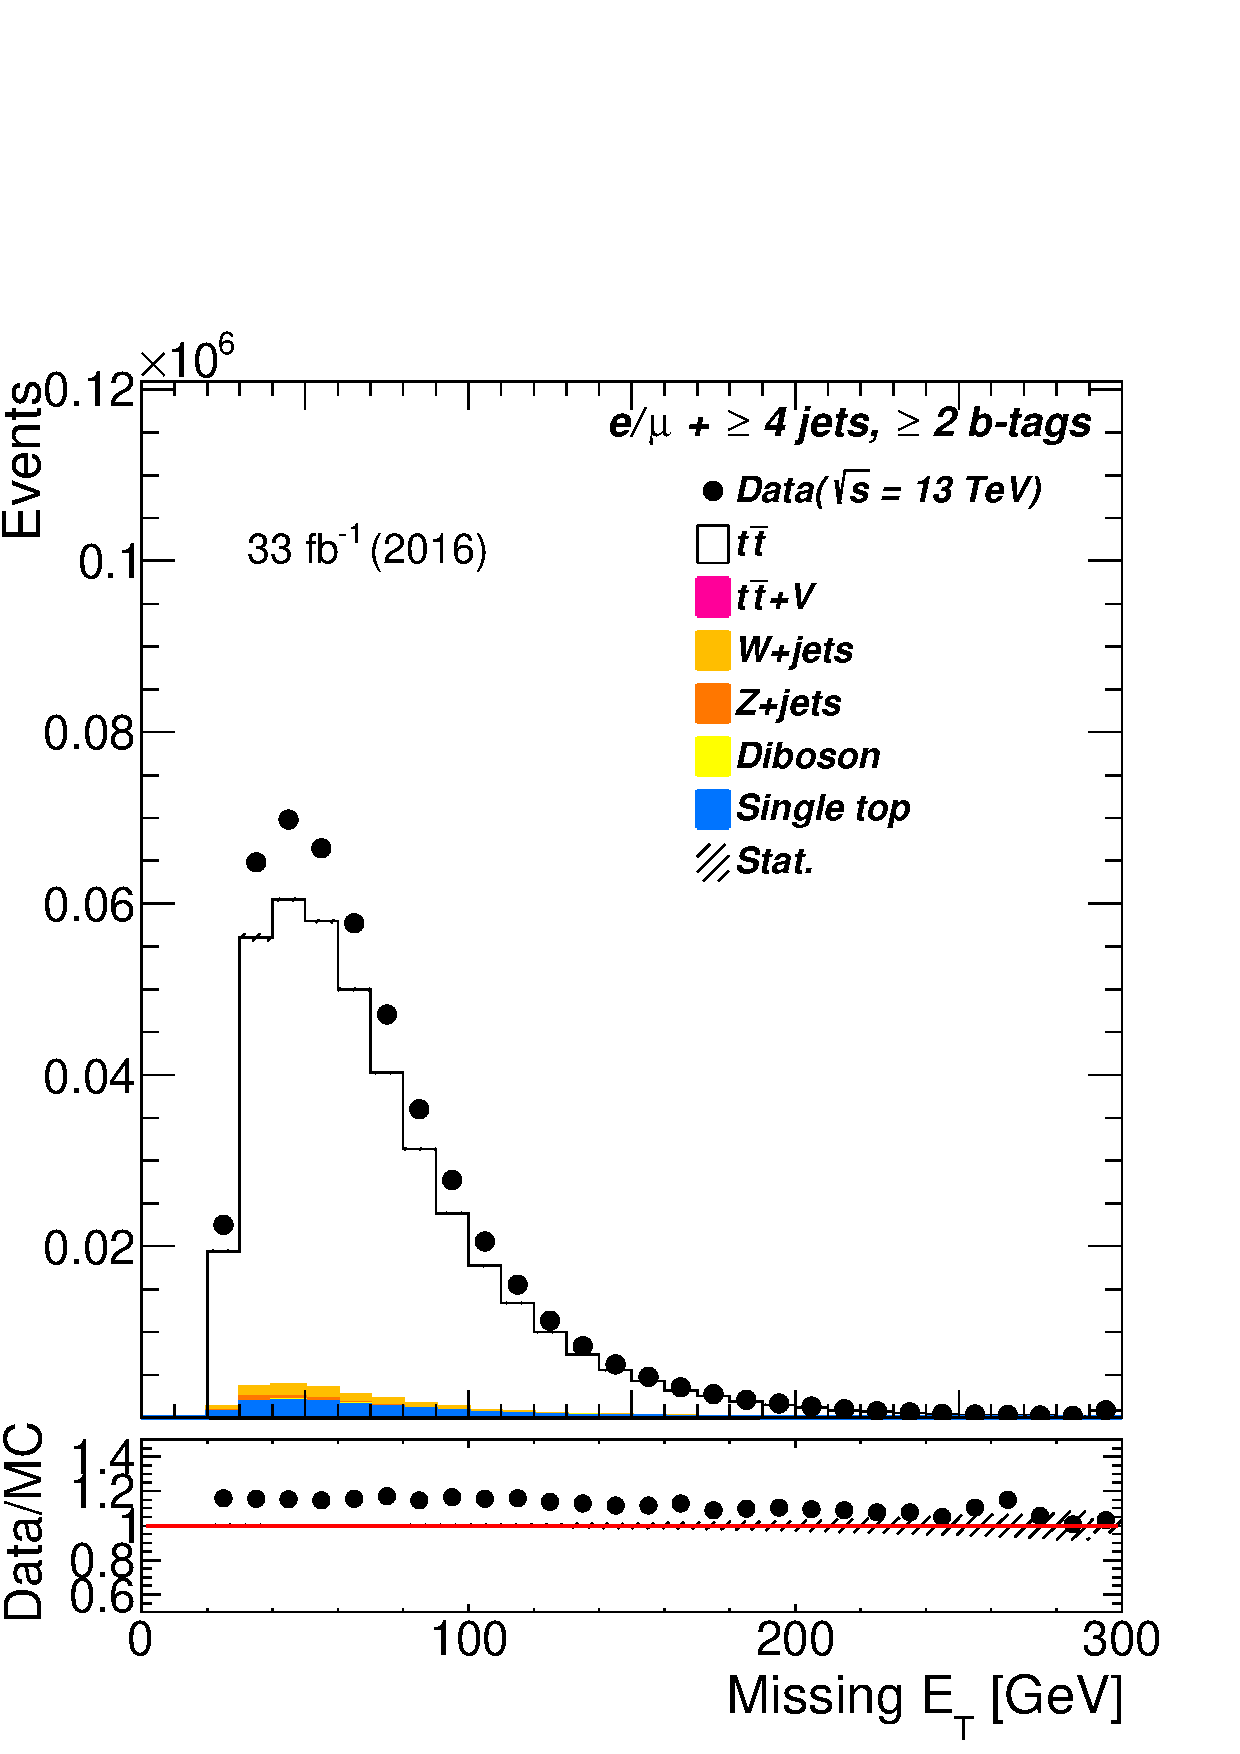
\includegraphics[width=\linewidth]{ControlPlots_emujets_2016_4incl_2incl/met_met_emujets_2016.png}
	 	\caption{$E_T^{\rm miss}$.} \label{fig:Sec5}
 \end{subfigure}
 \hspace*{0.5cm}
 	\begin{subfigure}{0.25\textwidth}
	 	\includegraphics[width=\linewidth]{ControlPlots_emujets_2016_4incl_2incl/met_phi_emujets_2016.png}
	 	\caption{$\phi$ of $E_T^{\rm miss}$.} \label{fig:Sec6}
	 \end{subfigure}

 
 

 \begin{subfigure}{0.25\textwidth}
 	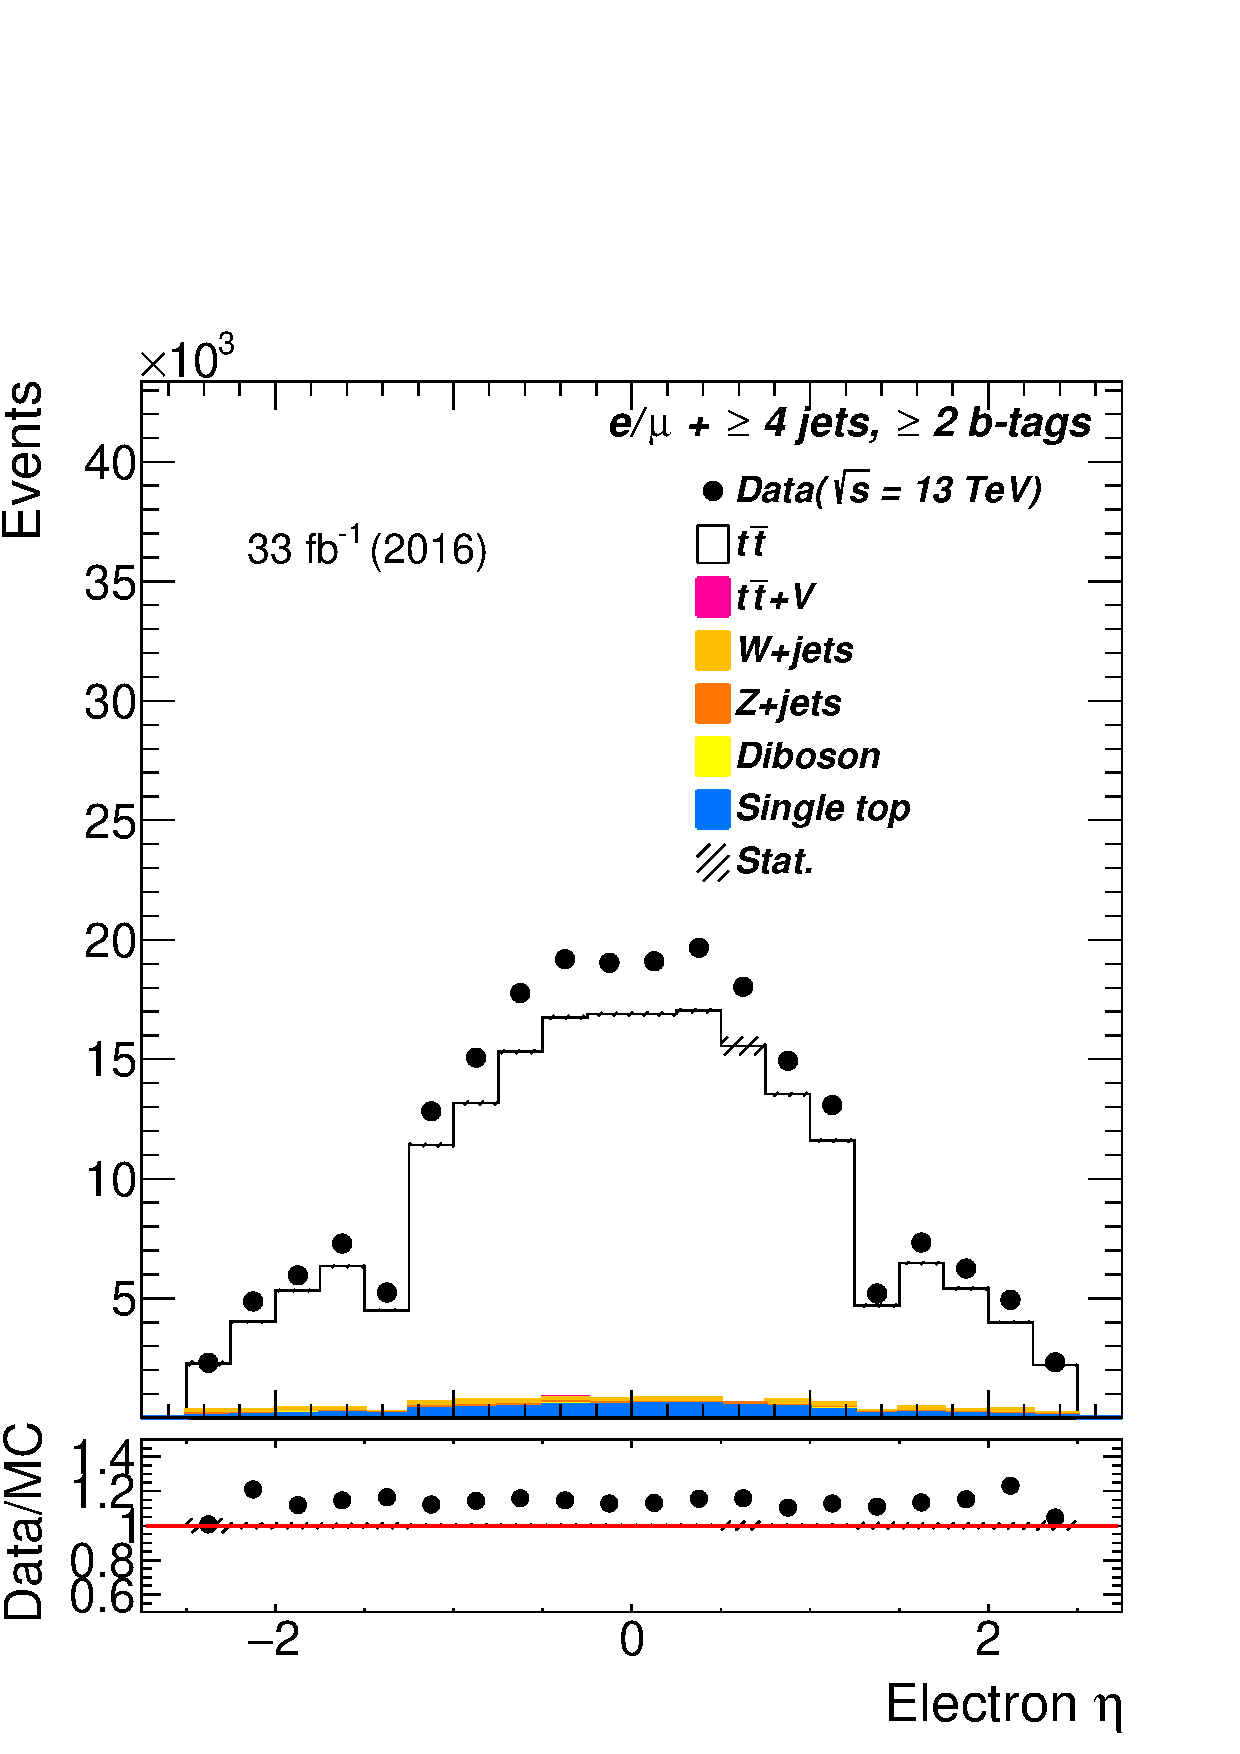
\includegraphics[width=\linewidth]{ControlPlots_emujets_2016_4incl_2incl/el_eta_emujets_2016.png}
 	\caption{$\eta$ of the electrons.} \label{fig:Sec9}
 \end{subfigure}\hspace*{0.5cm}
 \begin{subfigure}{0.25\textwidth}
 	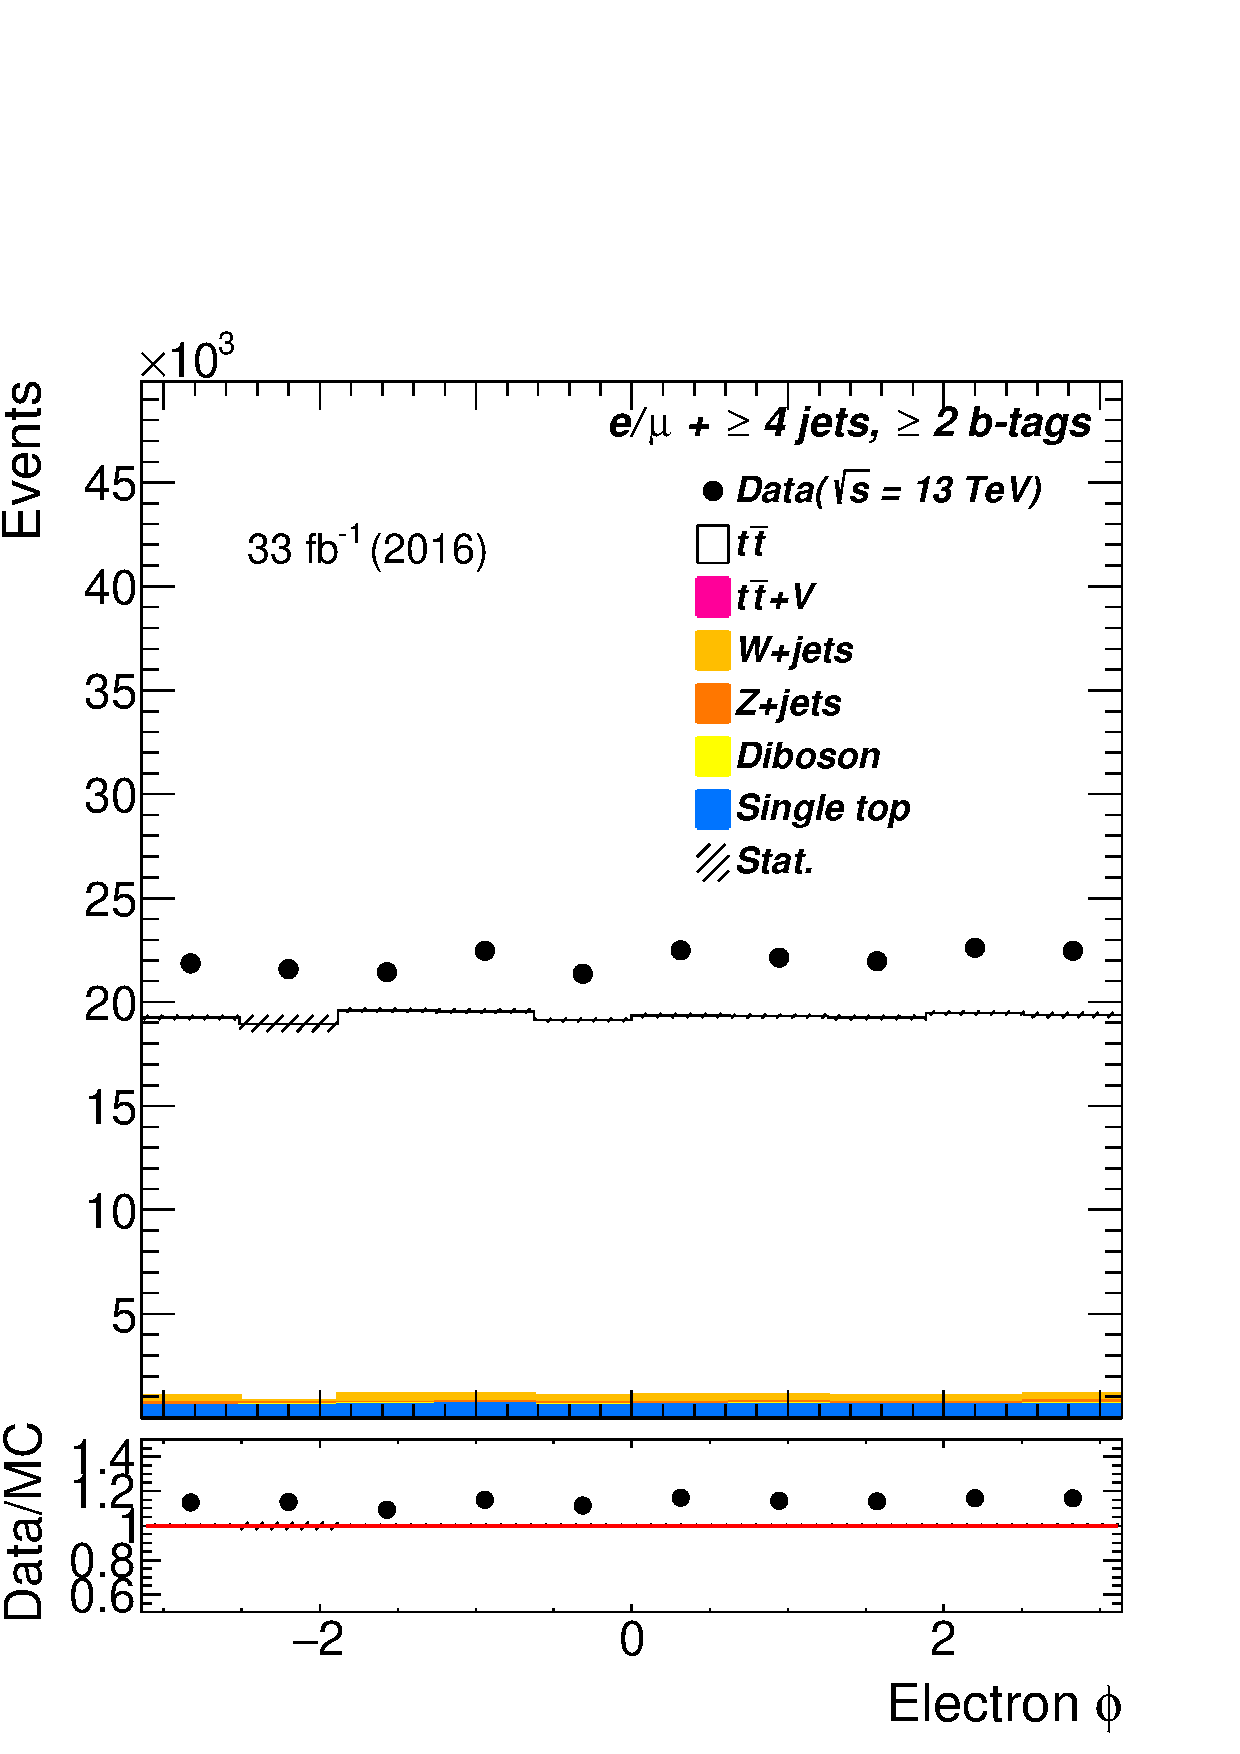
\includegraphics[width=\linewidth]{ControlPlots_emujets_2016_4incl_2incl/el_phi_emujets_2016.png}
 	\caption{$\phi$ of the electrons.} \label{fig:Sec10}
 \end{subfigure}\hspace*{0.5cm}
 \begin{subfigure}{0.25\textwidth}
 	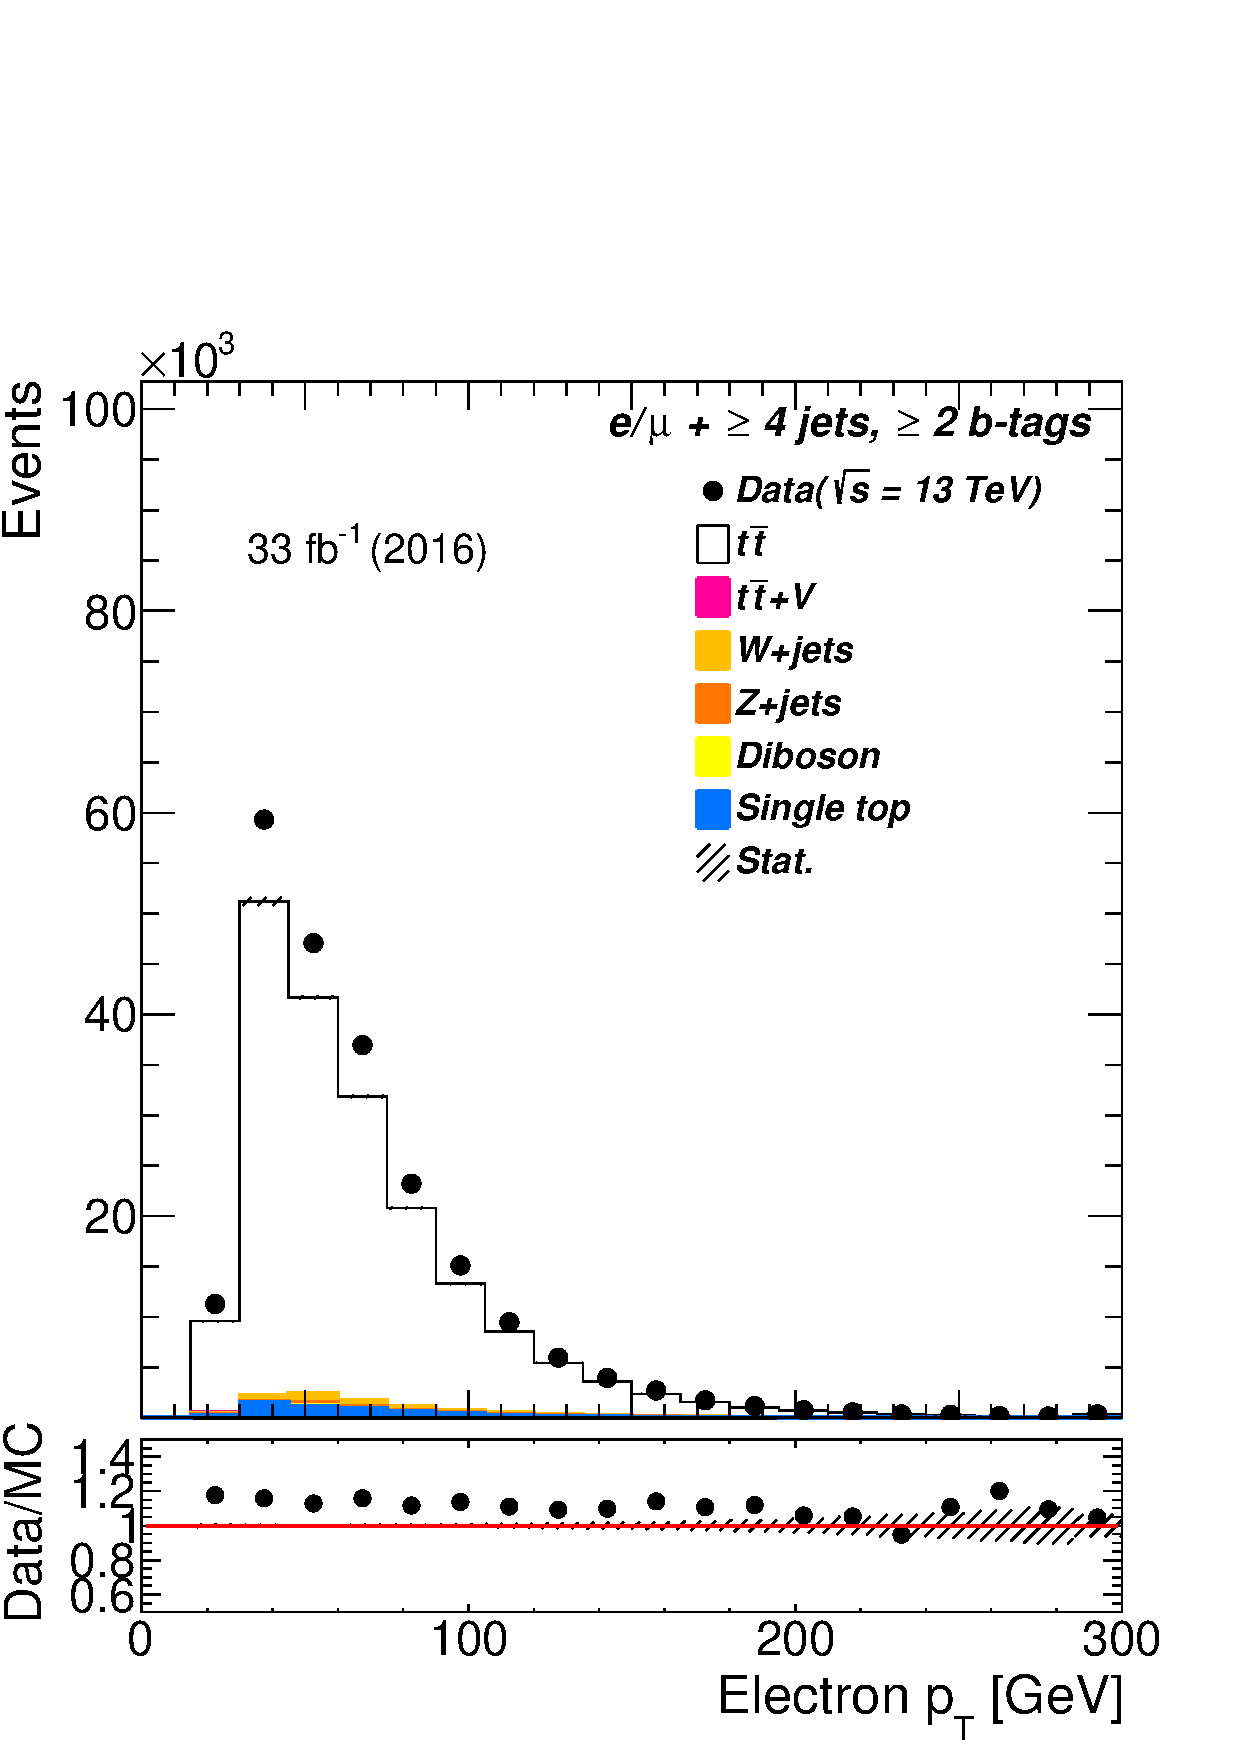
\includegraphics[width=\linewidth]{ControlPlots_emujets_2016_4incl_2incl/el_pt_emujets_2016.png}
 	\caption{Electron $p_T$.} \label{fig:Sec13}
 \end{subfigure}
 
 
 	
	\caption{Observed distributions after the event preselection. All events are observed in the lepton + jets decay channel and contain at least 4 jets and at least two $b$-tagged jets. The data is displayed by the black points. The solid histogram shows the signal-plus background predicted events, which are normalized to the number of events observed in data. The lower part shows the data-simulation agreement.}
	\label{fig:Sel1}
\end{figure}	


\begin{figure} % "[t!]" placement specifier just for this example
	\centering	


	\begin{subfigure}{0.25\textwidth}
	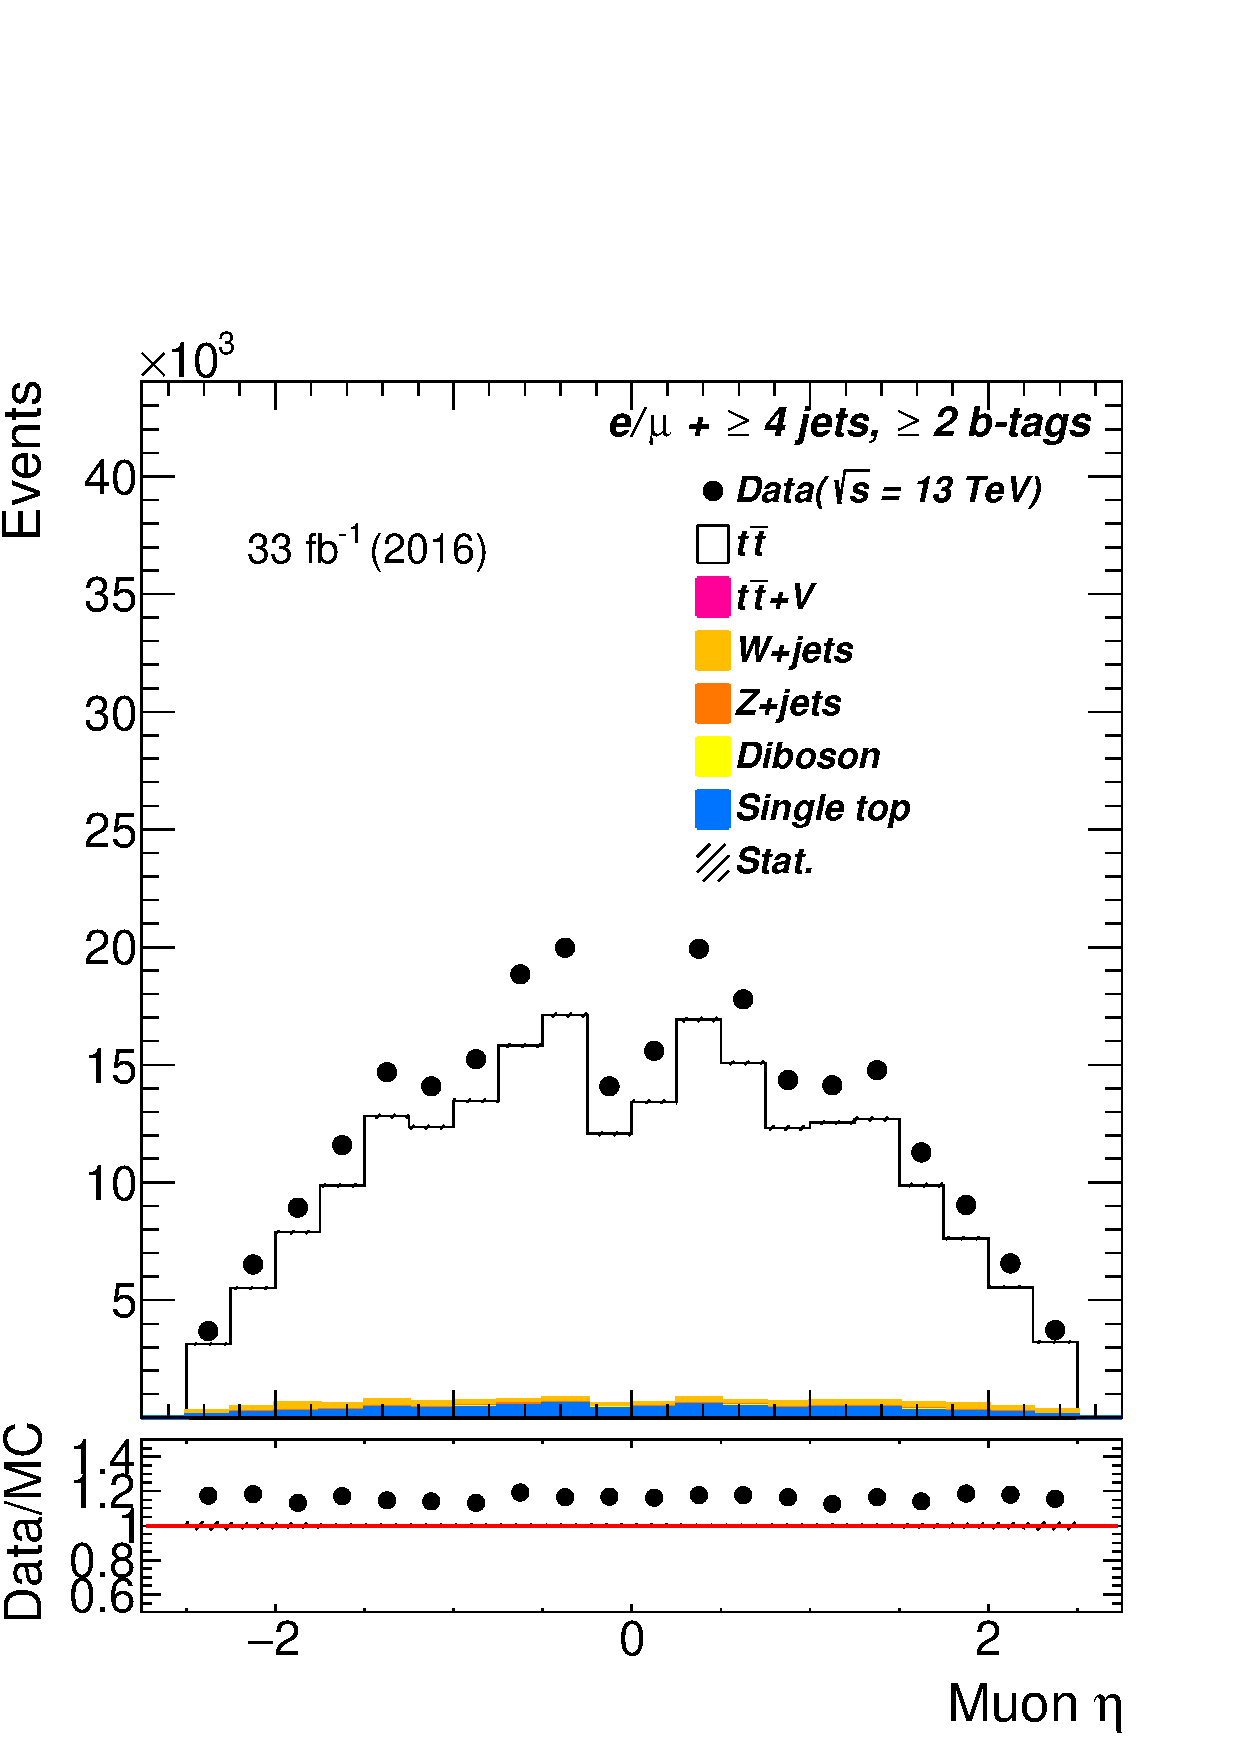
\includegraphics[width=\linewidth]{ControlPlots_emujets_2016_4incl_2incl/mu_eta_emujets_2016.png}
	\caption{$\eta$ the muons} \label{fig:Sec17}
\end{subfigure}\hspace*{0.5cm}
		\begin{subfigure}{0.25\textwidth}
	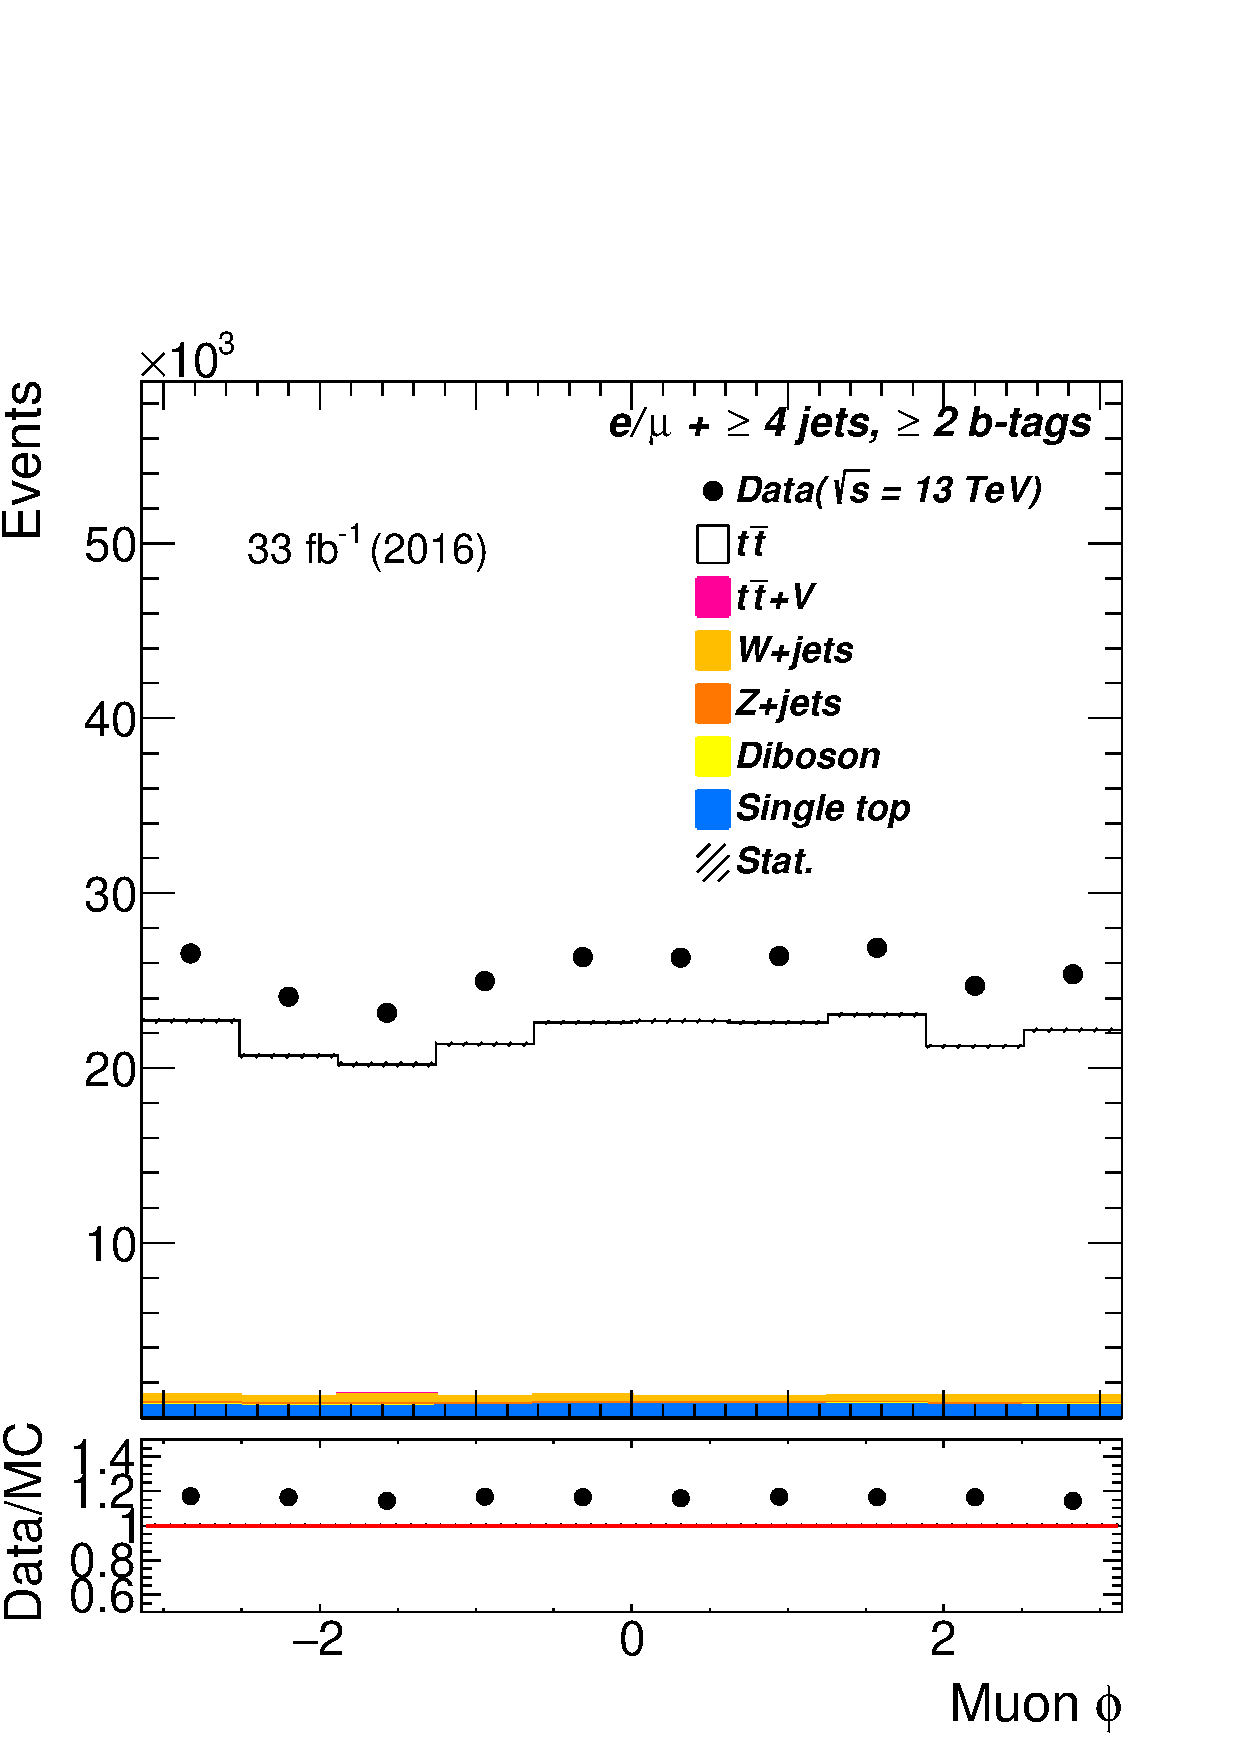
\includegraphics[width=\linewidth]{ControlPlots_emujets_2016_4incl_2incl/mu_phi_emujets_2016.png}
	\caption{$\phi$ of the muons.} \label{fig:Sec18}
\end{subfigure}\hspace*{0.5cm}
	\begin{subfigure}{0.25\textwidth}
		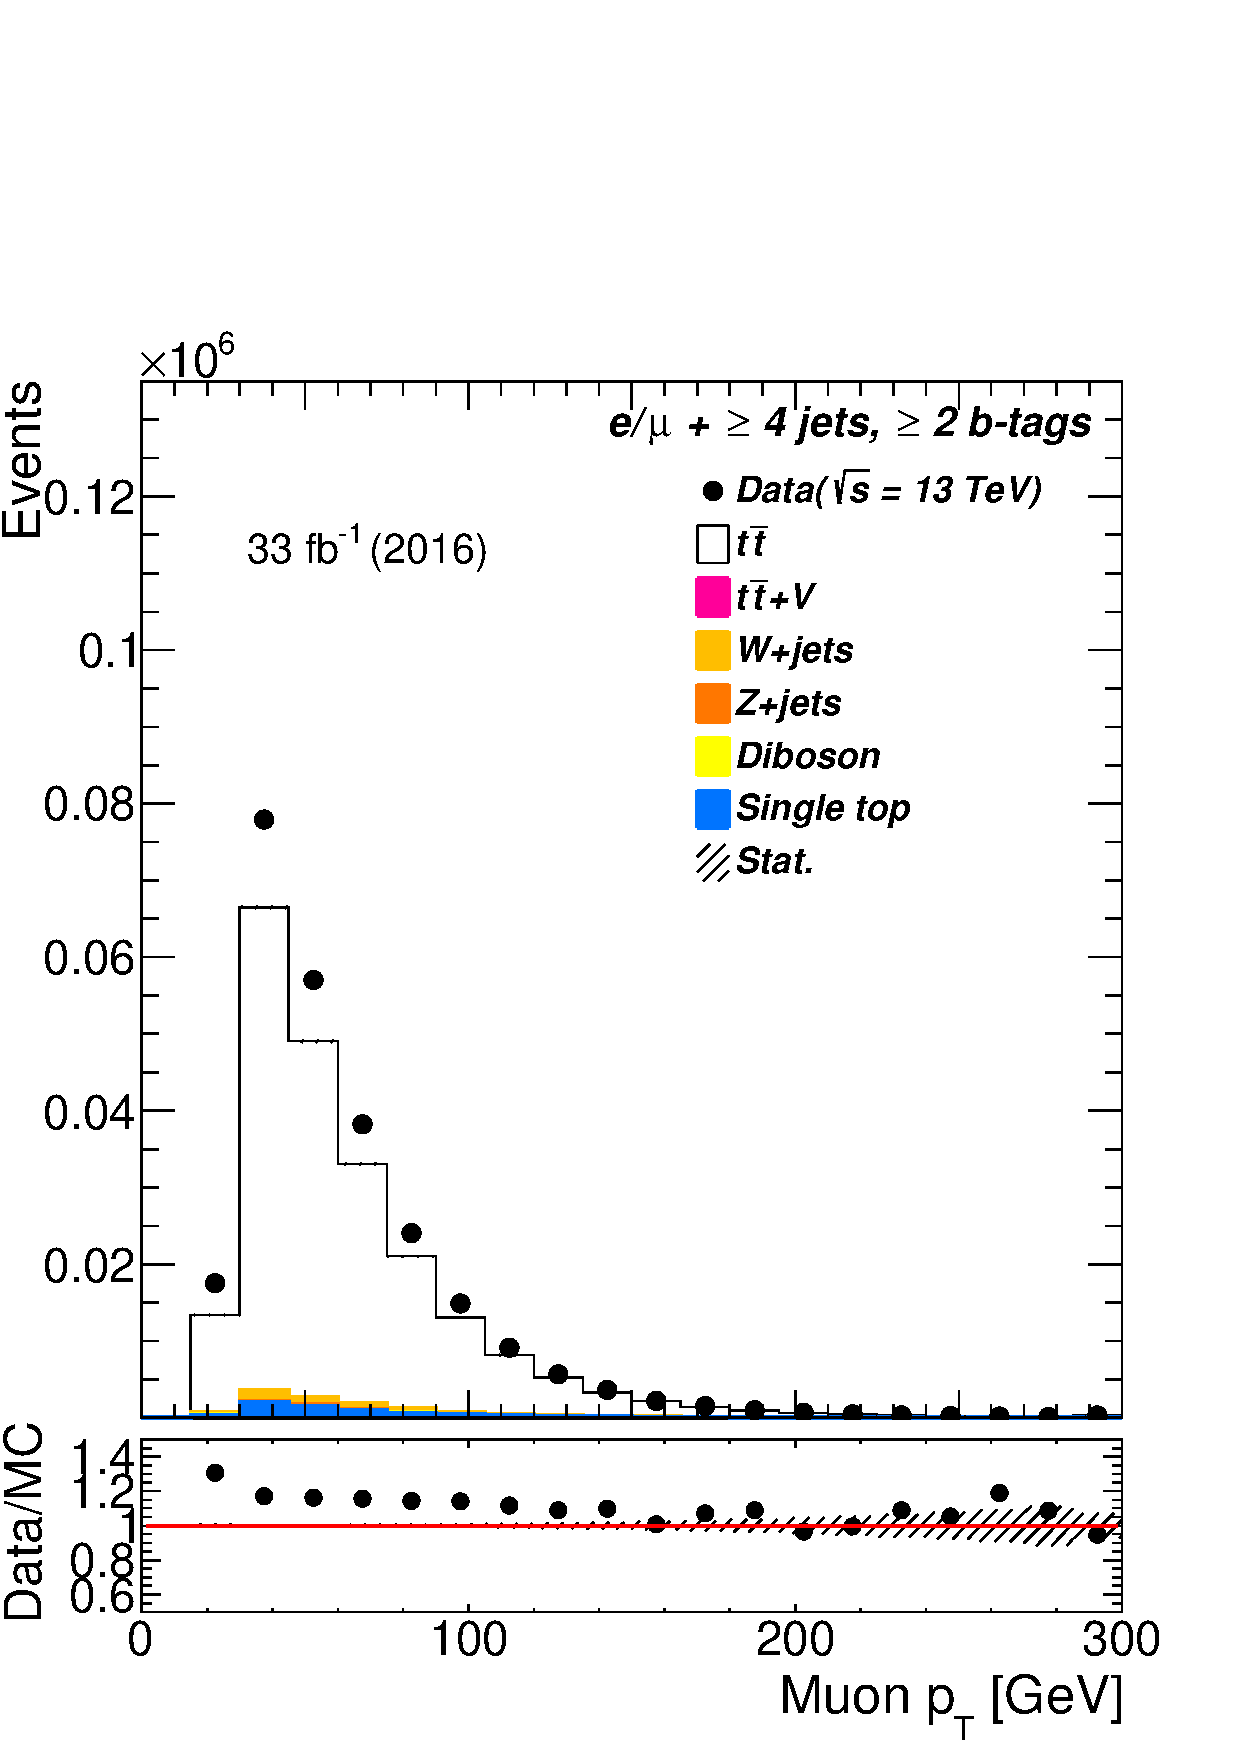
\includegraphics[width=\linewidth]{ControlPlots_emujets_2016_4incl_2incl/mu_pt_emujets_2016.png}
		\caption{Muon $p_T$.} \label{fig:Sec12}
	\end{subfigure}


	\begin{subfigure}{0.25\textwidth}
		\includegraphics[width=\linewidth]{ControlPlots_emujets_2016_4incl_2incl/jet0_eta_emujets_2016.png}
		\caption{$\eta$ the first jet.} \label{fig:Sec19}
	\end{subfigure}\hspace*{0.5cm}
\begin{subfigure}{0.25\textwidth}
	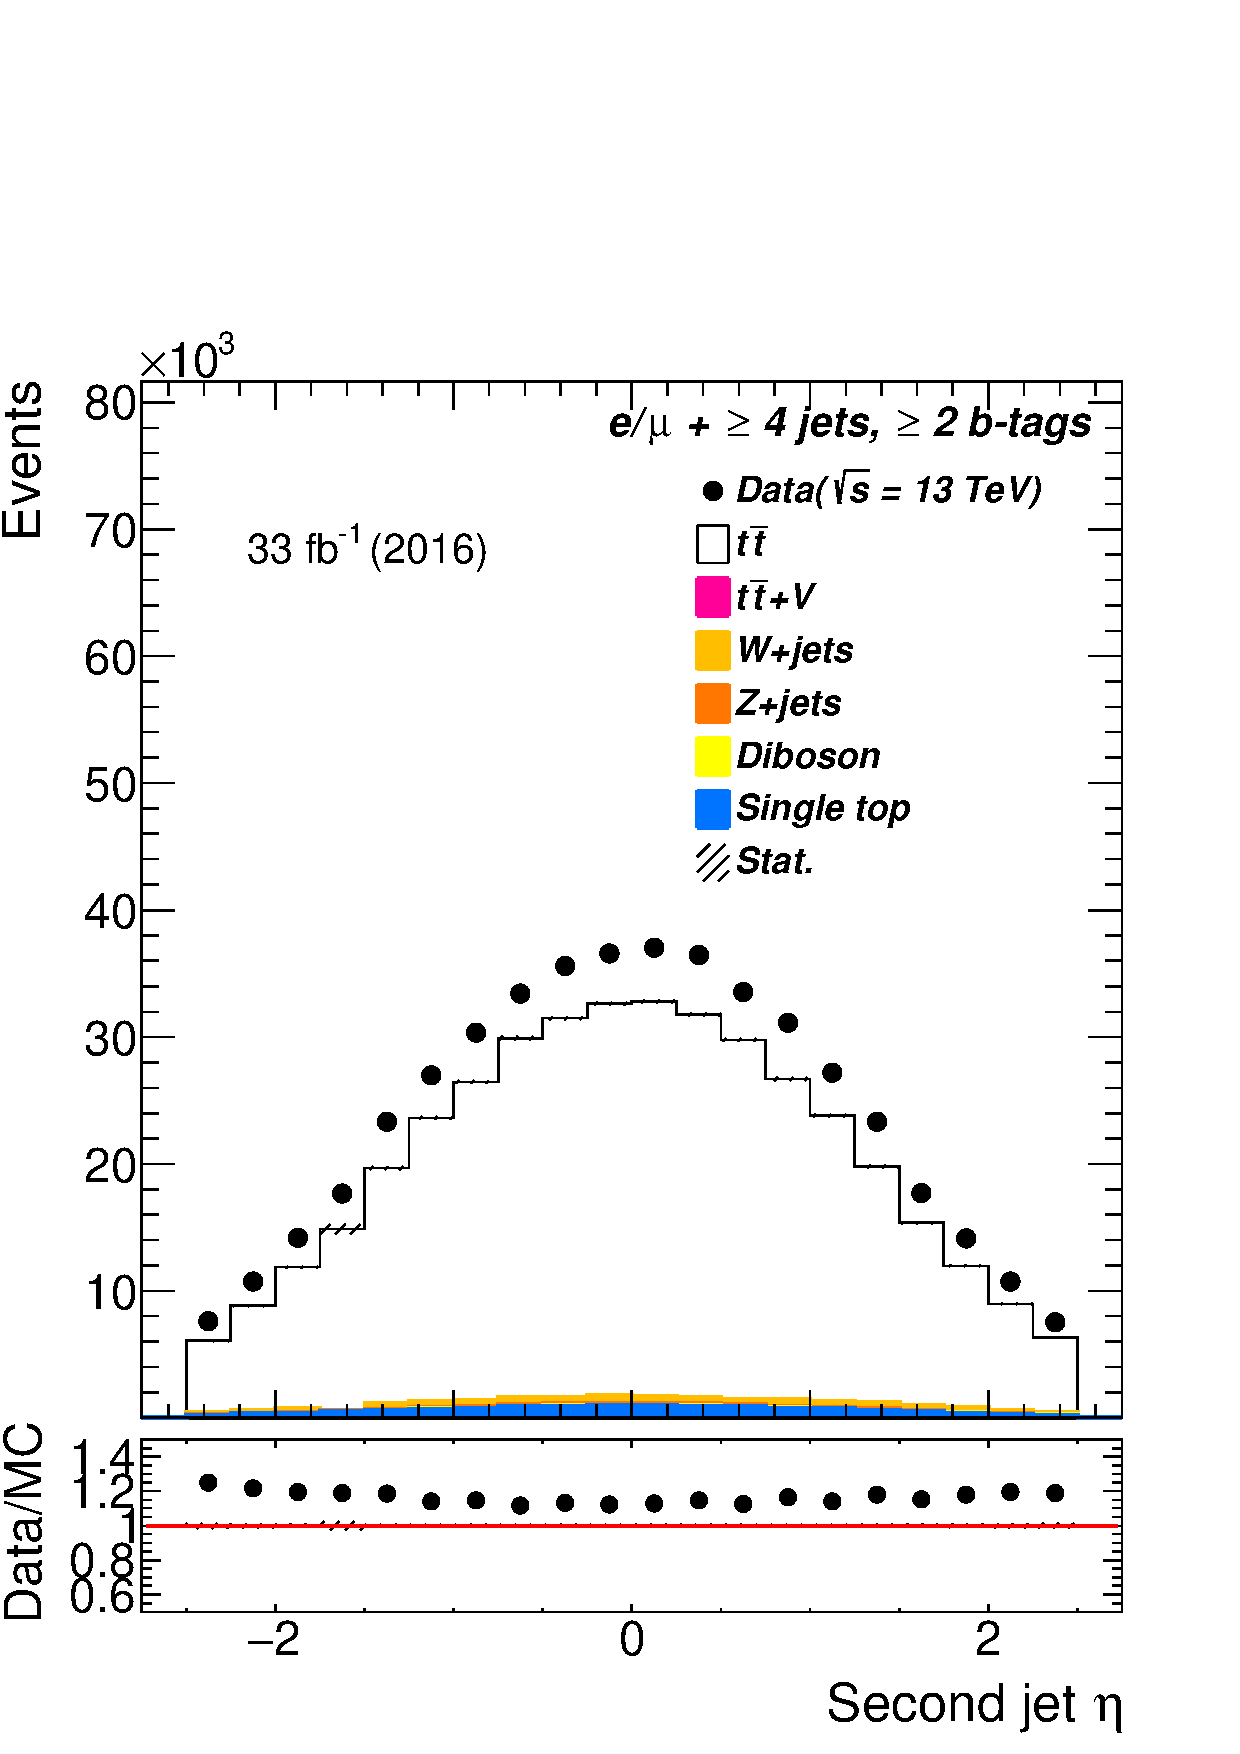
\includegraphics[width=\linewidth]{ControlPlots_emujets_2016_4incl_2incl/jet1_eta_emujets_2016.png}
	\caption{$\eta$ of the sec. jet.} \label{figSec23}
\end{subfigure}
\begin{subfigure}{0.25\textwidth}
	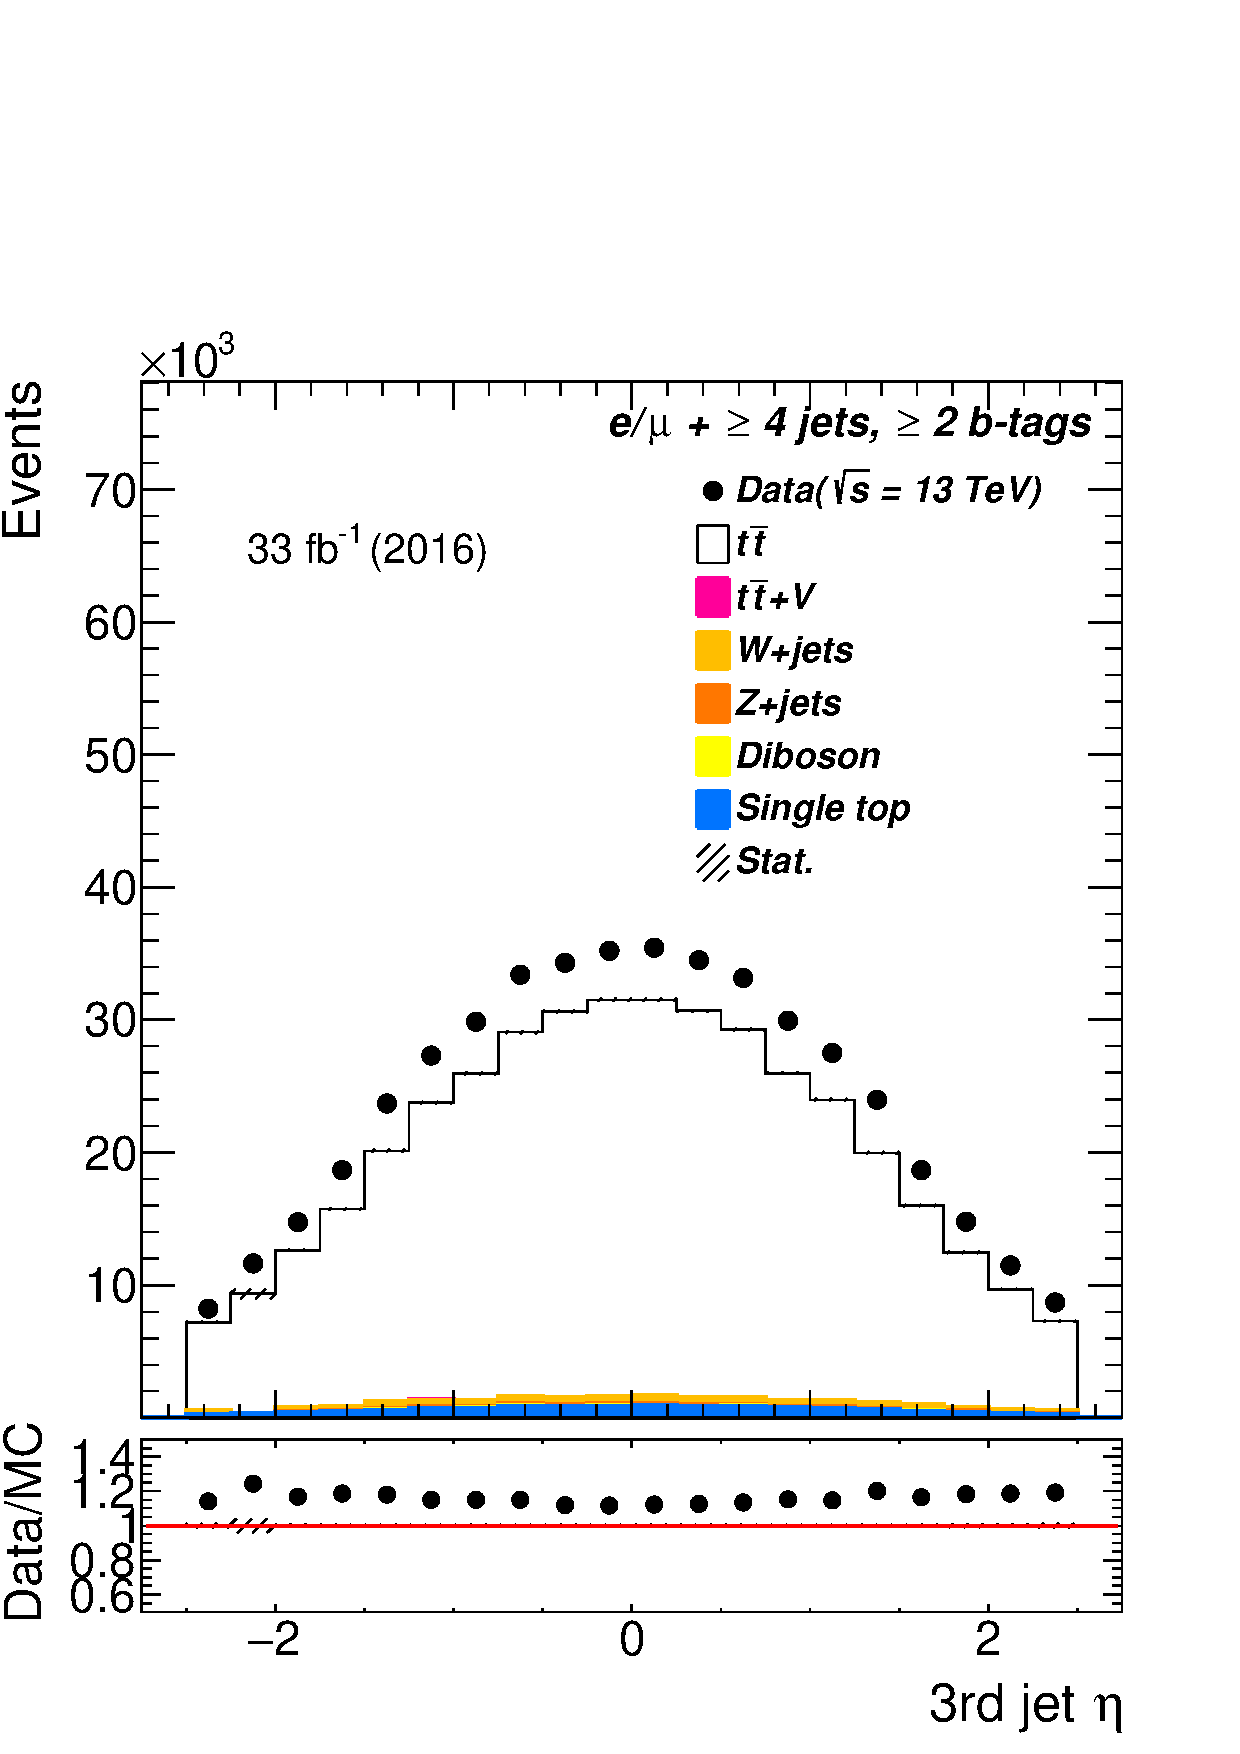
\includegraphics[width=\linewidth]{ControlPlots_emujets_2016_4incl_2incl/jet2_eta_emujets_2016.png}
	\caption{$\eta$ of the third jet.} \label{fig:Sec25}
\end{subfigure}

\begin{subfigure}{0.25\textwidth}
	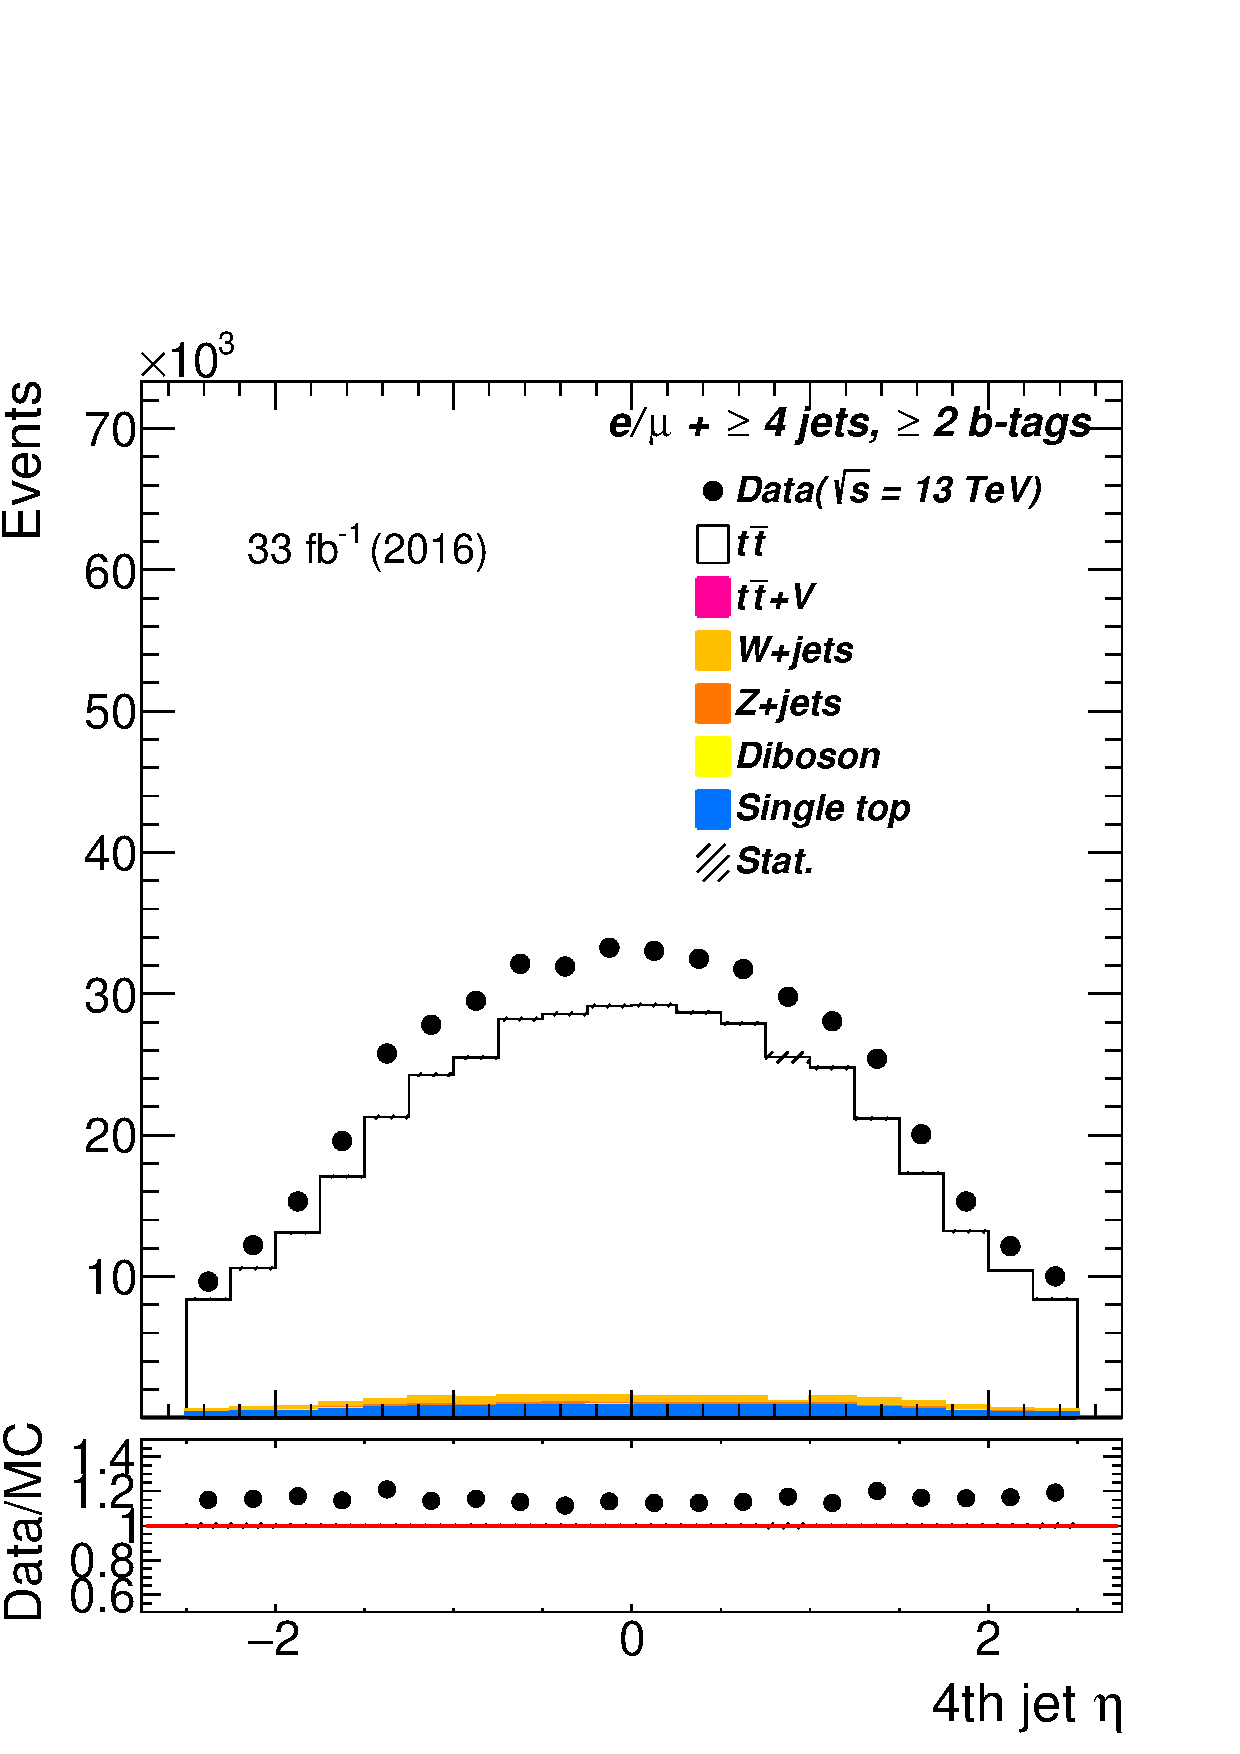
\includegraphics[width=\linewidth]{ControlPlots_emujets_2016_4incl_2incl/jet3_eta_emujets_2016.png}
	\caption{$\eta$ of the fourth jet.} \label{fig:Sec29}
\end{subfigure}



	
	\caption{As in~\cref{fig:Sel1}, global distributions are displayed for the muon, as well as for the four jets, obtained for the sample with at least 4 jets and at last two $b$-tagged jets.}	\label{fig:Sel2}
\end{figure}













